\section{Entwurf}
\label{sec:Entwurf}
In der Entwurfsphase sollen aus den Anforderungen Modelle der zu entwickelten Software entstehen, die die konkreten Hardware- und Softwarebezogenen Anforderungen berücksichtigen. Diese Modelle gelten dann als unmittelbare Vorlage für die sich anschließende Implementationsphase. (vgl. \cite[S. 69]{dumke-2003})

UML-Diagramme sind unter anderem ein effektives Werkzeug, um den Programm- und Datenentwurf zu unterstützen und zu dokumentieren. Letztendlich soll mithilfe geeigneter Modelle ein Entwurf der zu Implementierenden Software erarbeitet werden. Dies umfasst die Festlegung des Softwaredesignes, der Datenstruktur und der grafische Oberfläche.

\subsection{Logikentwurf}
\label{sec:Logikentwurf}
%TODO:MVVM
Der Logikentwurf soll basierend auf dem Use-Case-Diagramm, siehe Abbildung \ref*{fig:Use-Case-Diagramm} entstehen. Dabei sollen aus den Anwendungsfällen die benötigten Funktionen des Programms erarbeitet werden. Für einen ersten Überblick des gesamten Prozesses wurde ein Ablaufdiagramm erstellt was die Prozessschritte mit den benötigten Datenquellen zeigt, siehe Abbildung \ref*{abb:Flow}.

Die Anwendung soll als erstes den Nutzer authentifiezieren um die Berechtigungen feststellen zu können. Wenn der Nutzer berechtigt ist wird seine Referatszugehörigkeit mittels des AD ermittelt. Nach dem Login Prozess werdem dem Nutzer im Frontend die Anweseheitsdaten seiner Kollegen das aktuellen Monats angezeit. Dort kann er seine eigenen Anwesenheiten ändern oder in den Monatsansichten vor und zurück springen. Jede änderung eines eigenen oder im Falle eines Admins, eines Datensatzes im generellen wird direkt an die Datenbank übermittelt und dort gespeichert.

Um die einzelnen Prozessschritte als Funktionen näher zu beschreiben wurden Programmablaufpläne (PAP) erstellt. Beispielhaft ist im Anhang \ref{abb:PAP} der PAP für die Funktion des Änderns von Anwesenheiten.

\begin{figure}[htb]
    \centering
    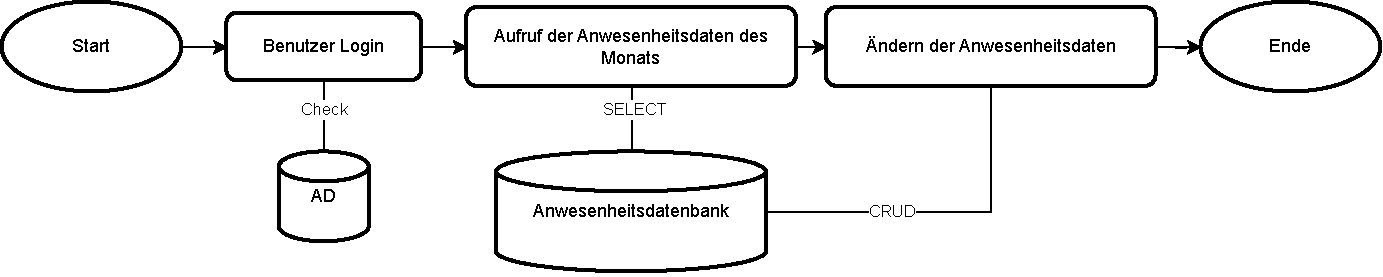
\includegraphics[width=0.9\textwidth,angle=0]{abb/Flow-Diagramm.drawio.pdf}
    \caption[Beschreibung]{Ablaufdiagramm}
    \label{abb:Flow}
\end{figure}




\subsection{Datenentwurf}
\label{sec:Datenentwurf}
Um die Daten aus dem Anwesenheitsplaner in eine Datenbank zu speichern muss dafür eine neue, mit passendem Schema, Angelegt werden. UML-Diagramme wie das ERM können dabei verwendet werden, um die Tabellenstruktur, die Beziehungen zwischen den Tabellen und die Attribute zu modellieren. Dies ermöglicht eine klare Darstellung der Datenbankstruktur und hilft dabei, die Datenintegrität und -konsistenz schon in der Planung sicherzustellen. Durch diese Art an Dokumentation ist es auch möglich bei der Entwicklung des Programms passende Klassen für die Verarbeitung der Daten aus der Datenbank herzuleiten.

Die zu speicherten Daten ergeben sich aus der in der Analysephase erhoben Tabelle im Abbildung \ref{abb:Ausgangstabelle}. Um die Daten möglichst simpel aus der Datenbank auslesen und zurückschreiben zu können, sollte versucht werden die Datenstruktur so anzulegen das die Daten in einem in der Programmlogik gut verarbeitbares Schema gespeichert werden. Um möglichst einfache Abfragen zu ermöglichen wurde keine Normalisierung der Tabellenstruktur durchgeführt um Zeit zu sparen. Um später Fehler zu vermeiden könnte das Schema für eine weiterentwicklung angepasst werden. Im aktuellen Fall wurde sich gegen eine Normalisierung entschieden, da die Prüfung der eingaben auf der Frontendseite geschehen soll.

Für das Anlegen der Datenstrukturen im Programmcode und in der Datenbank wurde ein Entity-Relationship-Modell (ERM), siehe \ref{abb:ERM} erstellt. Hier soll es zwei Tabellen geben, die Tabelle Person wird zum Teil aus dem AD befüllt und hält zum Teil Informationen die für Funktionen des Anwesenheitsplaners benötigt werden. Die Tabelle Anwesenheit beinhaltet alle Anwesenheitseinträge der Nutzer. Dem Nutzer wird eine ein Anwesenheitseintrag über die Verbindung mit seinem Sicherheitsbezeichner (SID) im AD zugeordnet. Die SID wird benötigt da sich der Name des Nutzers ändern kann und damit nicht als Primärschlüssel eignet. Die SID wird vom AD beim erstellen des Kontos angelegt und ändert sich nie. (vgl. \cite{sid})

\begin{figure}[htb]
    \centering
    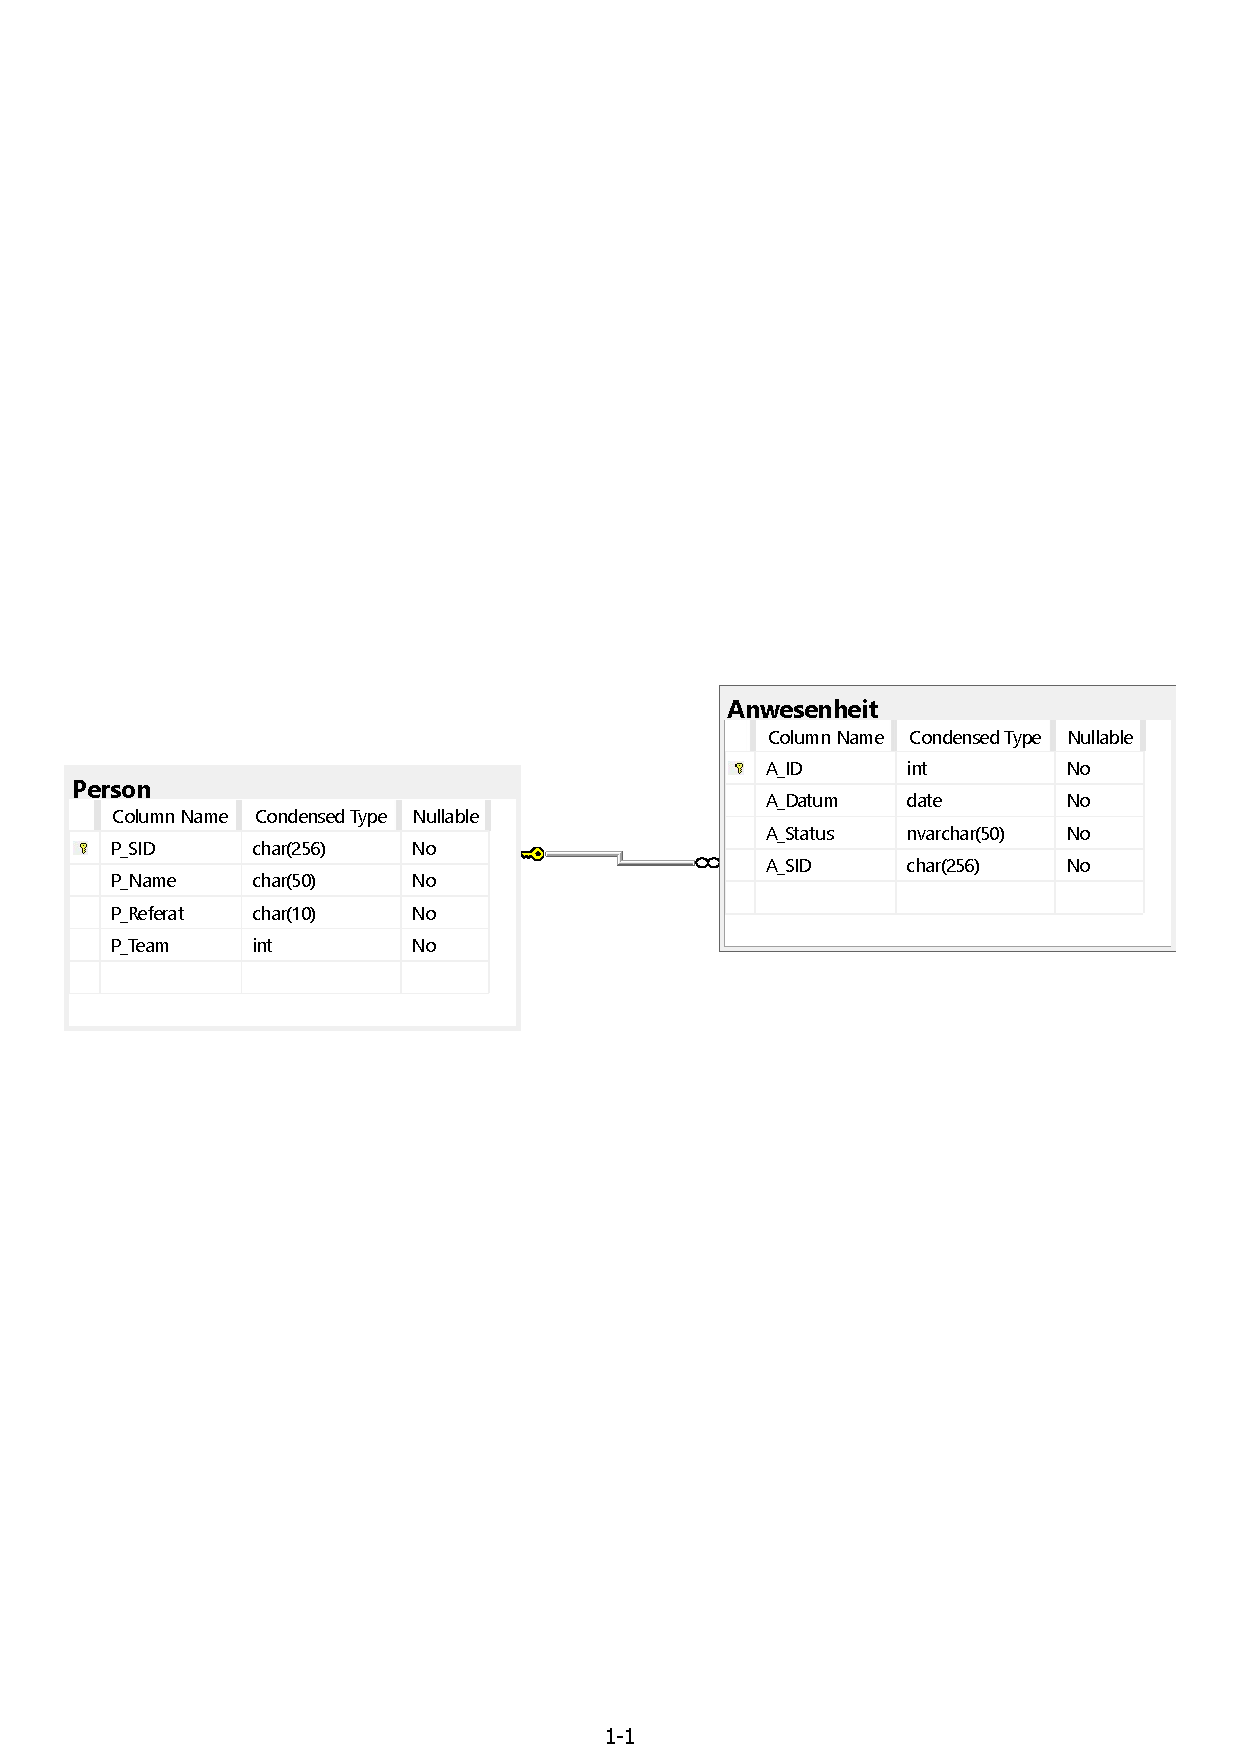
\includegraphics[width=0.9\textwidth,angle=0]{abb/ERM.pdf}
    \caption[Beschreibung]{ERM}
    \label{abb:ERM}
\end{figure}
%TODO:ERM erklären mit Quelle?

